\begin{figure}

\begin{subfigure}[t]{0.41\linewidth}
\centering
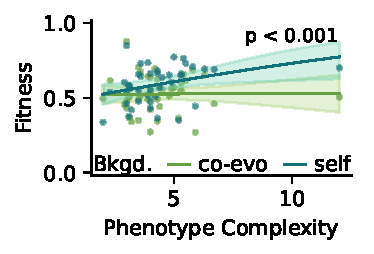
\includegraphics[width=\linewidth]{binder-2026-07-06-pcomplexity-gee.ipynb/binder/teeplots/2026-07-06-pcomplexity-gee/other=co-evo+viz=subplots+what=base+ext=.pdf}
\end{subfigure}%
\begin{subfigure}[t]{0.59\linewidth}
\centering
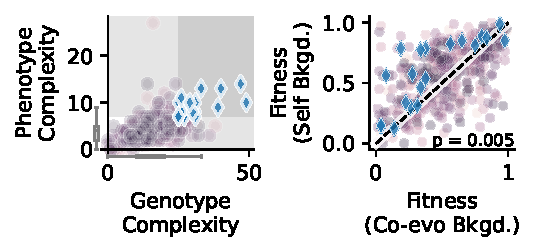
\includegraphics[width=\linewidth,trim={0.25cm 0 0 0},clip]{binder-2026-07-25-ecoselfcontext-pgcomplex-screen.ipynb/binder/teeplots/2026-07-25-ecoselfcontext-pgcomplex-screen/inner=box+iqr=shade+n=20+viz=subplots+ext=.pdf}
\end{subfigure}

\vspace{-4ex}

\begin{subfigure}[t]{0.37\linewidth}
\centering
\caption{\footnotesize niche construction selects for complexity }
\label{fig:general:gee-base}
\end{subfigure}%
\begin{subfigure}[t]{0.06\linewidth}
~
\end{subfigure}%
\begin{subfigure}[t]{0.57\linewidth}
\centering
\caption{\footnotesize niche construction is common in high-complexity strains }
\label{fig:general:pgcomplex-ecoself}
\end{subfigure}

% https://github.com/mmore500/oee4/blob/fa16a472ad6ac584ad7a5da7b7662729342ebc3b/binder/2026-07-25-ecoselfcontext-pgcomplex-screen.ipynb
% https://github.com/mmore500/oee4/blob/079d63f5e1583d71269a36cf9598431e4e34ac5e/binder/2026-07-06-pcomplexity-gee.ipynb
\caption{%
\textbf{Niche construction drives evolution of complexity across replicates.}
\footnotesize
Across original 100-stint replicates ($n=40$), fitness advantage of evolved complexity depends on self-acting selection (GEE, interaction coef. 0.145, $p < 0.001$; panel \ref{fig:general:gee-base}).
This relationship remains consistent after excluding case study strain (GEE, $p = 0.003$; Supplementary Figure \ref{TODO}) or disaggregating per-replicate point-in-time samples within replicates (autoregressive GEE; $p = 0.014$; Supplementary Figure \ref{TODO}).
Across additional 20-stint replicates ($n=400$), high-complexity replicates (top 5\% by genotype/phenotype complexity joint exceedance) disproportionately involve niche construction (Fisher's exact test, 18/2 vs. 216/164; $p = 0.004$); panel \ref{fig:general:pgcomplex-ecoself}).
This relationship remains consistent at 2.5\% and 7.5\% thresholds (9/1 vs. 225/165, $p=0.056$; 28/5 vs. 206/161, $p = 0.001$).
High-complexity replicates exhibit diverse morphologies, most differing from cigar morphology of case study (17/20; \url{https://hopth.ru/gz}).
}
\label{fig:general}
\end{figure}

\begin{figure}
\centering
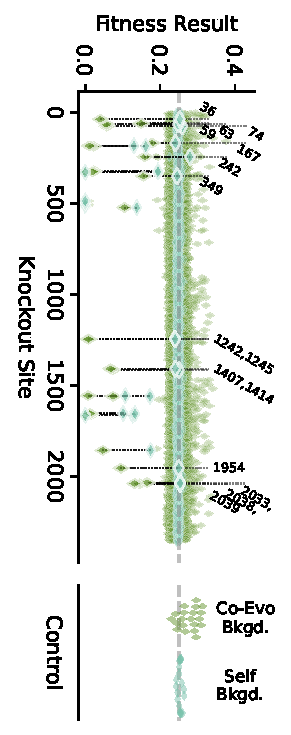
\includegraphics[height=0.9\linewidth,angle=90]{binder-2026-06-22-eco-gwas.ipynb/binder/teeplots/viz=subplots+ext=.pdf}

\vspace{-2ex}

% https://github.com/mmore500/oee4/blob/4a76b3624f7723879530f9b48310c96f8bc68b2a/binder/2026-06-22-eco-gwas.ipynb
\caption{%
\textbf{Case study strain selects for genotype complexity in co-evolved partner.}
\footnotesize
In stint-100 isolate of case study background strain, 14 genome sites exhibited strong adaptive benefit compared to single-site knockouts when tested with case study strain absent.
However, with case study strain present, adaptive benefit was detected at an additional 18 genome sites.
Co-evolutionary adaptation to case study strain thus accounts for 56\% (18/32) of detected genotype complexity in background strain.
}
\label{fig:general-supp:gwas}
\end{figure}
